\scanpage{105}
% L1
grâce au

% L2--3
\uline{Lemme} \quad a) Soit \deleted{$\unsure{E}$} $F$ (loc.) constructible dans $X$, \inserted{$E$ loc. const.} alors $F\cap E$ est (loc) constructible dans $E$

% L4--5
b) Soit \deleted{$\unsure{E}$} $F\subset E$, \inserted{avec $E$ (loc) constructible} alors $F$ est (loc.) constr. dans $E$ ssi il l'est dans $X$.

% L6--8
Dém. Pour a), on \unsure{montre|note} que si $F$ est ouvert rétrocompact dans $X$, alors $F\cap E$ est rétrocompact dans $E$, grâce au fait que tt ouvert \unsure{qu. cpt} $U$ de $E$ est
\diagram{\begin{tikzcd}[ampersand replacement=\&,row sep=small,column sep=small]
E\arrow[d,"f"] \& f^{-1}(F)\cap U\\
X \& F
\end{tikzcd}}
% L9--13
induit par un ouvert $V$ de $X$, qu'on peut si on veut [grâce à l'hyp \unsure{particulière|préliminaire} de la prop] supposer qu. cpt, d'où $f^{-1}(F)\cap U=f^{-1}(F\cap V)=$ image inverse d'un qu. cpt, qui est qu. cpt car $E$ est rétrocompact dans $X$, \deleted{\unsure{Donc|Dans}} \inserted{par $\unsure{0_{\mathrm{III}}|0_{\mathrm I}}$ 9.1.13.} Le cas ``localement''
% L14--16
en résulte aussitôt, utilisant le fait que $E$ induit un $E\cap U$ constructible dans \deleted{tt} $U$ ouvert\deleted{\unsure{e}}.

% L17--20
Pour b), on suppose $F\subset E$ constructible dans \uline{$E$} \inserted{\unsure{loc. ctr.|constr.}}, prouvons que $F$ l'est dans $X$. On peut supposer $F$ \deleted{\unsure{ouvert}} \deleted{fermé} \inserted{ouvert} dans $E$, rétrocompact dans $E$, \deleted{et} \inserted{\unsure{puis : et|puis : a)} cas} $E=U\cap \complement V$, $U$ et $V$ rétrocomp. \unsure{ds} dans $X$ \inserted{qui sont constructibles}
% L21--24
[car $E=\bigcup E_i$ réunion finie de tels, les \deleted{$F\cap E_i$ sont} dans \uline{$E$} par a), donc $E_i\cap F$ constr. dans $E_i$ par a), et on est ramené à prouver qu'ils sont constructibles dans $X$, puisque $F=\bigcup E_i\cap F$.
\margin{$0_{\unsure{\mathrm{II}|\mathrm{III}}}$ 9.1.8 \unsure{(i) b(ii)|(i) (ii)|(i) bis|(i)$\Rightarrow$(ii)}}
% L25--26
\deleted{\unsure{De sorte} $F$ \unsure{étant ouvert dans $E$, on} $F=$ \unsure{l'est-il|$E\cap W$}, \unsure{à fortiori dans} $X$, \unsure{donc}} \inserted{Remplaçant $X$ par $U$, on peut grâce à \deleted{\unsure{une hyp}} se borner au cas $X=U$ [$E$ étant constr. dans $U$\inserted{par \unsure{(i)|(ii)}}, $F$ \deleted{\unsure{donc|alors}} le sera dans $U$, donc dans $X$]}
% Large unlettered pen stroke in the lower left margin.
\figure{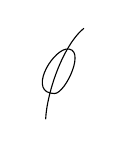
\begin{tikzpicture}[scale=.34]\draw (0,-1.6) .. controls (.05,-.6) and (.64,1.15) .. (1.43,1.8); \draw (.33,-.64) .. controls (-.65,-.63) and (.17,.89) .. (.76,1.02) .. controls (1.56,1.12) and (.75,-.64) .. (.33,-.64);\end{tikzpicture}}
% archive sheet number: 104
